\section{System Testing}

\subsection{Test Objectives and Environment}

Testing was conducted to evaluate the correctness of the library management functions, the coordination between system layers, main business workflows, and requirements regarding security and error handling. The scope focused on the Express/TypeScript backend, including modules for authentication, users, books, branches, document circulation, and AI features.\\

\textbf{Tools Used}
\begin{itemize}
        \item Jest combined with ts-jest to execute TypeScript test cases.
        \item Supertest to send HTTP requests to the Express application during integration and system testing.
        \item Mock Prisma Client and mocked external services for isolated testing, removing dependencies on live databases or email services.
        \item TypeScript Compiler with the \texttt{--noEmit} flag alongside Jest to verify source code quality.
\end{itemize}

\noindent Test source code is organized within the \texttt{backend-express/tests} directory, divided into four categories: \texttt{unit}, \texttt{integration}, \texttt{system}, and \texttt{quality}. Tests run in a Node.js environment and are configured centrally in the \texttt{jest.config.js} file.

\subsection{Unit Testing}

\textbf{Objectives} \\

Verify the correctness of individual functions or modules in isolation. Test cases focus on business logic, input validation, HTTP error codes, token verification, password handling, and exception branches. Prisma Client, mailer, and external dependencies are replaced with mocks so that results remain unaffected by the execution environment.\\

\noindent \textbf{Methodology} \\

Each function is tested against valid, invalid, boundary, and exception cases. Key functional groups include registration and login, OTP verification, book management, patron management, document circulation, authentication middleware, and error normalization.

\begin{table}[H]
\centering
\caption{Scope and Results of Unit Testing}
\begin{tabularx}{\textwidth}{|p{4.2cm}|X|c|c|}
\hline
\textbf{Test Group} & \textbf{Main Content} & \textbf{Suites} & \textbf{Result} \\
\hline
Auth and DTO & Registration, OTP, login, input validation & 3 & Pass \\
\hline
Books & Book CRUD, book utilities, catalog management & 3 & Pass \\
\hline
Users and Branches & Patron profiles, branch business logic & 2 & Pass \\
\hline
Circulation and Middleware & Borrow/return, auth middleware, error handling & 3 & Pass \\
\hline
\multicolumn{2}{|r|}{\textbf{Total}} & \textbf{10} & \textbf{168/168} \\
\hline
\end{tabularx}
\end{table}

The example below tests the scenario of registering with an already existing email. The expected result is that the service returns an HTTP 409 error and does not create a new account.

\begin{lstlisting}[language=R, caption={Unit test case for registration feature}]
it('returns 409 when email already exists', async () => {
    prismaMock.user.findUnique.mockResolvedValueOnce({ id: 'exists' });

    await expect(authService.register({
        email: 'reader@example.com',
        password: 'password1',
        fullName: 'A',
    })).rejects.toMatchObject({ statusCode: 409 });
});
\end{lstlisting}

Unit testing results show that 10/10 test suites passed, corresponding to 168/168 test cases passed. Code coverage for this group reached 94.33\% statements, 77.58\% branches, 94.44\% functions, and 95.07\% lines. \\

\begin{figure}[H]
    \centering
    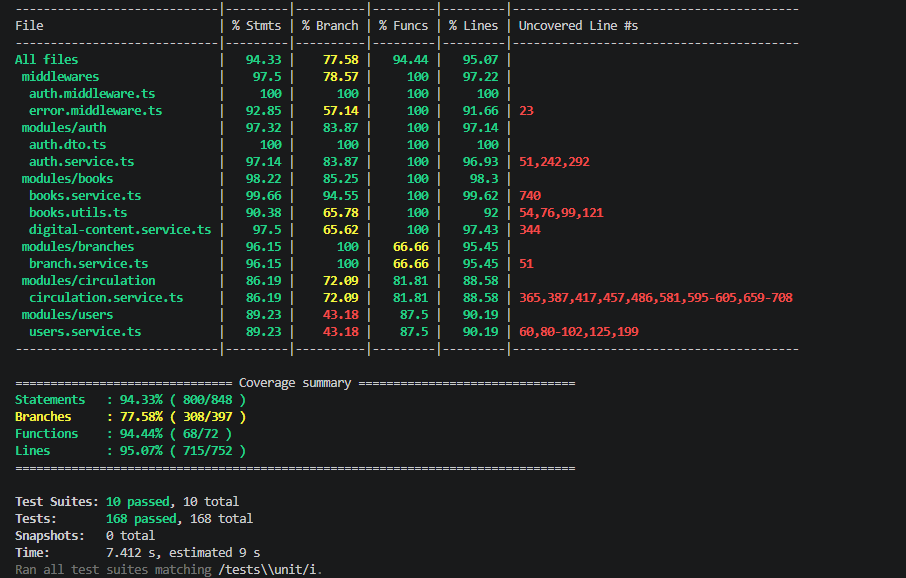
\includegraphics[width=0.9\textwidth]{Images/unit_test_result.png}
    \vspace{0.5cm}
    \caption{Unit test results}
    \label{fig:unit-test-result}
\end{figure}

\subsection{Integration Testing}

\textbf{Objectives} \\

Verify the coordination between routes, middleware, controllers, services, and the data access layer through actual HTTP requests sent to the Express application. This testing suite confirms response structures, HTTP status codes, authentication mechanisms, and inter-functionality integration within the same module.\\

\noindent \textbf{Methodology} \\

Supertest is used to simulate GET, POST, PATCH, and DELETE requests. The Prisma Client is mocked at the data boundary, while the Express application is fully instantiated so that routes and middleware execute just as they would in a live environment.

\begin{table}[H]
\centering
\caption{Scope and Results of Integration Testing}
\begin{tabularx}{\textwidth}{|p{4.2cm}|X|c|c|}
\hline
\textbf{API/Module} & \textbf{Tested Content} & \textbf{Suites} & \textbf{Result} \\
\hline
Auth & Registration, OTP verification, login, payload errors & 1 & Pass \\
\hline
Books and Branches & Book lookup, catalog and branch management & 2 & Pass \\
\hline
Users and Circulation & User profiles, borrowing, returning, renewals & 2 & Pass \\
\hline
AI Service & Interacting with AI service endpoints & 1 & Pass \\
\hline
\multicolumn{2}{|r|}{\textbf{Total}} & \textbf{6} & \textbf{67/67} \\
\hline
\end{tabularx}
\end{table}

The example below tests the login API with valid credentials. In addition to HTTP status 200, the test confirms that the response payload includes an access token, refresh token, and user profile details.

\begin{lstlisting}[language=R, caption={Integration test case for login API}]
const response = await request(app)
    .post('/api/v1/auth/login')
    .send({ email: 'reader@library.edu.vn', password: 'CorrectPass@123' });

expect(response.status).toBe(200);
expect(response.body.success).toBe(true);
expect(response.body.data.accessToken).toBeDefined();
expect(response.body.data.refreshToken).toBeDefined();
\end{lstlisting}

Integration testing achieved 6/6 passing test suites and 67/67 passing test cases. All evaluated endpoints returned status codes and response bodies appropriate for both success and error scenarios. \\

\begin{figure}[H]
    \centering
    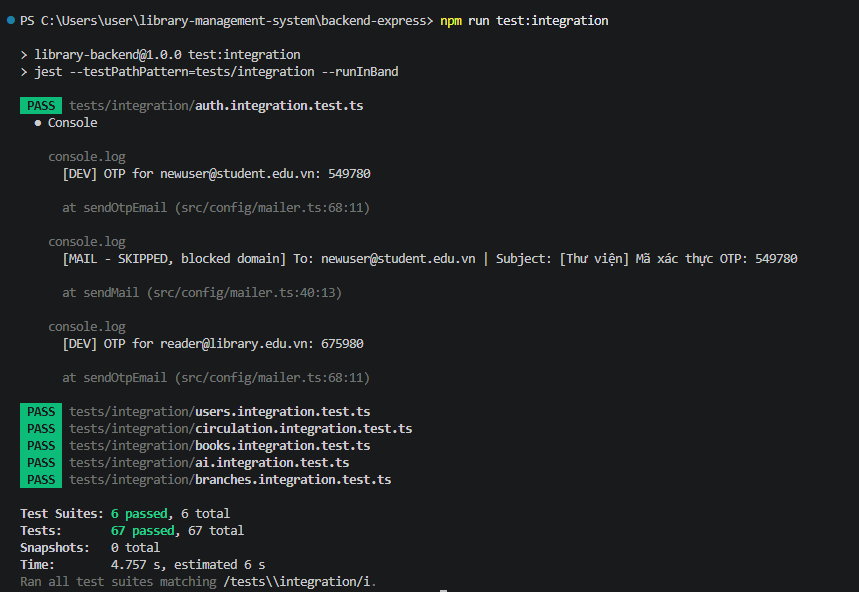
\includegraphics[width=0.9\textwidth]{Images/integration_test_result.png}
    \vspace{0.5cm}
    \caption{Integration test results}
    \label{fig:integration-test-result}
\end{figure}


\subsection{System Testing}

\textbf{Objectives} \\ 

Validate end-to-end business workflows from user requests to final system outputs. This group focuses on the patron lifecycle, borrow--renew--return cycles, reservation queues, overdue fine calculation, and authorization security.\\

\noindent \textbf{Methodology}\\

Business steps are simulated in real-world sequential order. Each step sends a request using the appropriate user role and verifies both the returned response and updated business state. The security testing group includes edge cases for missing tokens, expired tokens, tampered tokens, unauthorized role access, security headers, and non-existent endpoints.

\begin{table}[H]
\centering
\caption{System Testing Workflows}
\begin{tabularx}{\textwidth}{|p{5cm}|X|c|}
\hline
\textbf{Business Workflow} & \textbf{Tested Content} & \textbf{Result} \\
\hline
Patron Lifecycle & Registration, verification, profile update, account usage & Pass \\
\hline
Document Circulation & Book addition, search, borrowing, history viewing, renewal, return & Pass \\
\hline
Reservations and Queues & Item reservation, queue ordering, readiness notifications & Pass \\
\hline
Overdue Fines & Overdue identification, fine creation, payment handling & Pass \\
\hline
System Security & JWT, RBAC, Helmet, 404 errors, invalid JSON payloads & Pass \\
\hline
\multicolumn{1}{|r|}{\textbf{Total}} & \textbf{5 test suites, 36 test cases} & \textbf{36/36} \\
\hline
\end{tabularx}
\end{table}

For example, the circulation workflow sequentially checks a librarian adding a book, a patron searching for it, the librarian creating a borrow record, and the patron requesting a renewal. The case below verifies that the librarian role is authorized to create a borrow record:

\begin{lstlisting}[language=R, caption={System test case for book borrowing workflow}]
const response = await request(app)
    .post('/api/v1/circulation/borrow')
    .set(roleAuthHeader(Role.LIBRARIAN, librarianId))
    .send({ userId: readerId, barcode: copyBarcode });

expect(response.status).toBe(201);
expect(response.body.success).toBe(true);
expect(response.body.data.borrowRecordId).toBe(borrowRecordId);
\end{lstlisting}

Results show that all 5 system workflows passed, with 36/36 test cases succeeding. Cases involving missing tokens, invalid tokens, unauthorized access, and malformed JSON payloads were correctly rejected with appropriate HTTP status codes. \\

\begin{figure}[H]
    \centering
    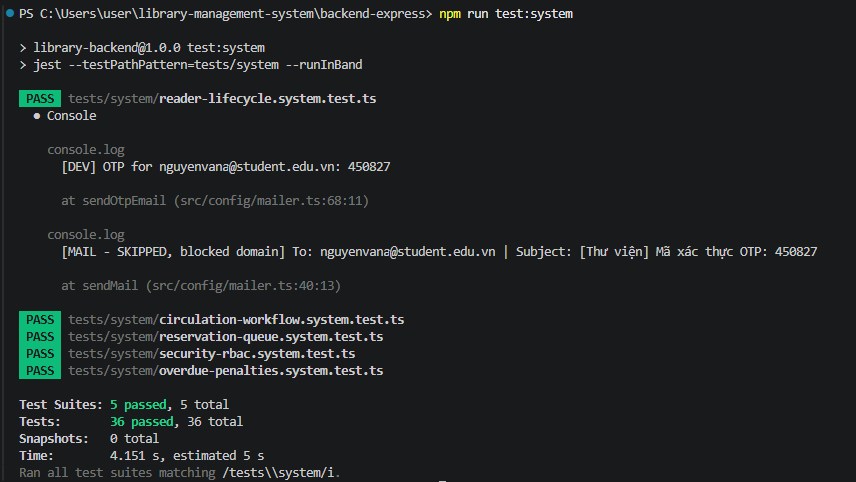
\includegraphics[width=0.9\textwidth]{Images/system_test_result.png}
    \vspace{0.5cm}
    \caption{System test results}
    \label{fig:system-test-result}
\end{figure}

\subsection{Code Quality Testing}

\textbf{Objectives} \\

Evaluate static quality conditions and architectural conventions in addition to functional testing. Verification topics include TypeScript compilation, source directory integrity, hardcoded secret detection, route--service layering, API response structures, and normalized error codes.\\

\noindent \textbf{Methodology} \\ 

Tests parse and analyze TypeScript files within the \texttt{src} directory while executing \texttt{npx tsc --noEmit}. Criteria are expressed as Jest assertions so that any violation is automatically caught within the testing pipeline.

\begin{table}[H]
\centering
\caption{Source Code Quality Test Results}
\begin{tabularx}{\textwidth}{|p{6cm}|X|c|}
\hline
\textbf{Criterion} & \textbf{Tested Content} & \textbf{Result} \\
\hline
TypeScript Compilation & Entire backend compiles without type errors & Pass \\
\hline
Codebase Integrity & The \texttt{src} directory exists; TypeScript files are non-empty & Pass \\
\hline
Security & No hardcoded passwords, JWT secrets, or connection strings & Pass \\
\hline
Layered Architecture & Routes do not invoke Prisma directly; controllers forward errors via \texttt{next} & Pass \\
\hline
Responses and Error Codes & Normalized \texttt{success} property and valid HTTP status codes & Pass \\
\hline
\multicolumn{1}{|r|}{\textbf{Total}} & \textbf{2 test suites, 10 test cases} & \textbf{10/10} \\
\hline
\end{tabularx}
\end{table}

\begin{figure}[H]
    \centering
    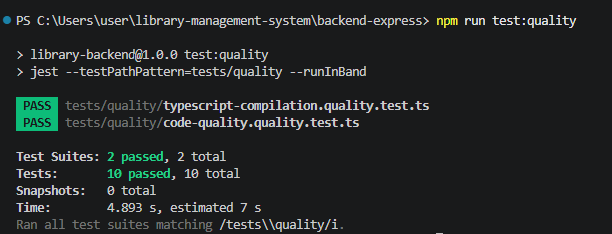
\includegraphics[width=0.9\textwidth]{Images/quality_test_result.png}
    \vspace{0.5cm}
    \caption{Quality test results}
    \label{fig:quality-test-result}
\end{figure}

\subsection{Test Summary}

All backend tests were executed using the command \texttt{npm test -- --runInBand}. The overall summary is presented in Table~\ref{tab:test-summary}.

\begin{table}[H]
\centering
\caption{Backend Test Summary}
\label{tab:test-summary}
\begin{tabular}{|l|r|r|r|}
\hline
\textbf{Test Type} & \textbf{Test Suites} & \textbf{Test Cases} & \textbf{Passed} \\
\hline
Unit & 10 & 168 & 168 \\
\hline
Integration & 6 & 67 & 67 \\
\hline
System & 5 & 36 & 36 \\
\hline
Code Quality & 2 & 10 & 10 \\
\hline
\textbf{Total} & \textbf{23} & \textbf{281} & \textbf{281} \\
\hline
\end{tabular}
\end{table}

\noindent All 23 test suites executed successfully with zero failing test cases and no snapshot tests. These results confirm that key functionality, cross-layer coordination, security rules, and source code quality standards of the backend satisfy all test requirements at the time of evaluation. \\

\begin{figure}[H]
    \centering
    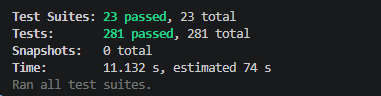
\includegraphics[width=0.9\textwidth]{Images/summary_test_result.png}
    \vspace{0.5cm}
    \caption{Summary of test results}
    \label{fig:summary-test-result}
\end{figure}